\documentclass[aspectratio=169]{beamer}

\input{../ceesd-macros.tex}
\usepackage[absolute, overlay]{textpos}

% Define a new environment for a code snippet box
\newtcolorbox{codebox}[1][]{
  colback=white,
  colframe=black!75!black,
  width=\linewidth,
  arc=4pt,
  outer arc=4pt,
  left=6pt,
  right=6pt,
  boxsep=5pt,
  #1
}

\newtcolorbox{fancycode}[3][]{
  colback=white,
  colframe=black!75!black,
  width=0.8\linewidth,
  arc=1pt,
  outer arc=1pt,
  left=1pt,
  right=1pt,
  top=1pt,
  bottom=1pt,
  boxsep=0pt,
  overlay={
    % Draw the tab
    \draw[fill=white, rounded corners=1mm] 
      ([xshift=-0.5cm, yshift=2pt]frame.north east) --
      ([yshift=2pt]frame.north east) --
      (frame.north east) --
      ([xshift=-0.5cm]frame.north east) -- cycle;
    % Add the source link
    \node[anchor=north east, font=\tiny, text=black] 
      at ([xshift=-0.25cm, yshift=1pt]frame.north east) {Source: \href{#2}{\texttt{#3}}};
  },
  #1
}

% Define a new tcolorbox environment for the code block
\newtcolorbox{codeblock}[3][]{
  colback=white,
  colframe=black!75!black,
  width=0.8\linewidth,
  arc=1pt,
  outer arc=1pt,
  left=1pt,
  top=1pt,
  bottom=1pt,
  right=1pt,
  boxsep=0pt,
  overlay={
    \node[anchor=south east, font=\tiny, text=black] at (frame.south east) {Source: \href{#2}{\texttt{#3}}};
  },
  #1
}

\newtcolorbox{emptyblock}[2][]{
  colback=white,
  colframe=black!75!black,
  width=0.8\linewidth,
  arc=1pt,
  outer arc=1pt,
  left=1pt,
  top=1pt,
  bottom=1pt,
  right=1pt,
  boxsep=0pt,
  overlay={
    % Draw the tab
    \draw[fill=white, draw=black!75!black, rounded corners=1mm] 
      ([xshift=-1cm, yshift=1cm]frame.north east) rectangle ++(1cm, 0.5cm);
    % Add the text
    \node[anchor=north east, font=\tiny, text=black] 
      at ([xshift=-0.5cm, yshift=1.25cm]frame.north east) {#2};
  },
  #1
}
\newcommand{\blockwithtab}[2]{
  \begin{tikzpicture}
    % Draw the box
    \node[anchor=north west, draw=black!75!black, fill=white, rounded corners=1mm, text width=0.8\linewidth, inner sep=5pt] (box) {#1};
    % Draw the tab
    \node[anchor=south east, draw=black!75!black, fill=white, rounded corners={1mm,1mm,0mm,0mm}, text width=1cm, inner sep=2pt, yshift=0.5pt] at (box.north east) {#2};
  \end{tikzpicture}
}

%\newcommand{\blockwithtab}[2]{
%  \begin{tikzpicture}
%    % Draw the box
%    \node[anchor=north west, draw=black!75!black, fill=white, rounded corners=1mm, text width=0.8\linewidth, inner sep=5pt] (box) {#1};
%    % Draw the tab
%    \node[anchor=south, draw=black!75!black, fill=white, rounded corners=1mm, text width=1cm, inner sep=2pt, yshift=2pt] at (box.north east) {#2};
%  \end{tikzpicture}
%}
%\newcommand{\blockwithtab}[3][]{
%  \begin{tikzpicture}
%    % Draw the box
%    \node[anchor=north west, draw=black!75!black, fill=white, rounded corners=1mm, text width=0.8\linewidth, inner sep=5pt] (box) {#3};
%    % Draw the tab
%    \node[anchor=south, draw=black!75!black, fill=white, rounded corners=1mm, text width=1cm, inner sep=2pt, yshift=2pt] at (box.north east) {#2};
%  \end{tikzpicture}
%}

% Kaushik's code listings
% Taken from https://www.overleaf.com/learn/latex/code_listing
\definecolor{codegreen}{rgb}{0,0.6,0}
\definecolor{codegray}{rgb}{0.5,0.5,0.5}
\definecolor{codepurple}{rgb}{0.58,0,0.82}
\definecolor{backcolour}{rgb}{0.95,0.95,0.92}
\lstdefinestyle{kkcodestyle}{
    language=python,
    backgroundcolor=\color{backcolour},
    commentstyle=\color{codegreen},
    keywordstyle=\color{magenta},
    numberstyle=\tiny\color{codegray},
    stringstyle=\color{codepurple},
    basicstyle=\ttfamily\footnotesize,
    breakatwhitespace=false,
    breaklines=true,
    captionpos=b,
    keepspaces=true,
    showspaces=false,
    showstringspaces=false,
    aboveskip=0pt,
    belowskip=0pt,
    showtabs=false,
    tabsize=2,
    escapeinside=@@
}

% Luke Olson's definition box
\newtcolorbox{lukedef}[1][Definition:]{
colback=white,
colbacktitle=white,
coltitle=IllinoisOrange,
colframe=IllinoisBlue,
boxrule=1pt,
titlerule=0pt,
%arc=15pt,
title={\strut#1},
}

% Matt's code listings
\definecolor{mintedlikecommentcolor}{rgb}{0.16,0.51,0.51}
\definecolor{mintedlikekeywordcolor}{rgb}{0,0.6,0}
\definecolor{mintedlikestringcolor}{rgb}{0.79,0,0}
\newcommand{\mintedlikebasicstyle}[1]{\ttfamily#1\linespread{4}}
\lstdefinestyle{mintedlike}{
    language=python,
    basicstyle=\mintedlikebasicstyle{\normalsize},
    commentstyle=\itshape\color{mintedlikecommentcolor},
    keywordstyle=\color{mintedlikekeywordcolor},
    stringstyle=\color{mintedlikestringcolor},
    columns=fullflexible,
    breakatwhitespace=false,
    breaklines=false,
    keepspaces=true,
    showspaces=false,
    showstringspaces=false,
    showtabs=false,
    tabsize=4,
    belowskip=-0.6\baselineskip,
    escapeinside=&&
}
% End MJS Additions


\newtcolorbox{codeblock2}[1][]{
  colback=white,
  colframe=black!75!black,
  width=0.8\linewidth,
  arc=1pt,
  outer arc=1pt,
  left=1pt,
  right=1pt,
  top=1pt,
  bottom=0pt,
  boxsep=0pt,
  #1
}

\newcommand{\codeblockwithtab}[2]{
  \begin{tikzpicture}
    % Draw the tab
    \node[draw, fill=white, rounded corners=1mm, anchor=south east] 
      at (0.8\linewidth, 0.5cm) {Source: \href{#1}{\texttt{#2}}};
    % Draw the code block
      \node[anchor=north west] at (0,0) {
        \begin{codeblock2}
         \lstinputlisting[style=kkcodestyle, basicstyle=\tiny, language=Python]{Figures/mtc/rhs_sample.py}
        \end{codeblock2}
      };
  \end{tikzpicture}
}
\newcommand{\snippetbox}[2]{
  \begin{tikzpicture}
    % Draw the box
    \node[draw=black!75!black, fill=white, rounded corners=1mm, text width=0.8\linewidth, inner sep=5pt, anchor=north west] (box) {
        \lstinputlisting[style=kkcodestyle, basicstyle=\tiny, language=Python]{#1}
    };
    
    % Draw the tab
    \draw[thin, rounded corners=1mm] (box.north east) -- ++(0,0.3) -- ++(-1,0) [rounded corners=0mm] -- ++(0,-0.3) -- cycle;
    \node[font=\tiny] at ([xshift=-0.5cm, yshift=1.5mm] box.north east) {#2};    % Draw the tab
    % \draw[thick, rounded corners=1mm] (box.north east) -- ++(0,0.5) -- ++(-1,0) [rounded corners=0mm] -- ++(0,-0.5) -- cycle;
    % \node[font=\tiny] at ([xshift=-0.5cm, yshift=2.25mm] box.north east) {#2};
  \end{tikzpicture}
}


%\newif\ifmovies
%\moviestrue
%\moviesfalse

%\newif\ifsubs
%\substrue
%\subsfalse

\newif\ifnotes
\notestrue
%\notesfalse


\begin{document}

% %======================================================================
% \begin{frame}\frametitle{04 --- Simulations }
% \setcounter{framenumber}{0}


% \vspace*{0.3in}
% {
%   \tiny
%   \textbf{Details on full-system simulation status including a discussion of integration of the
%     necessary physics modules and scaling of the present code.}

%   You should address the following:
%   \begin{itemize}
%   \item The goals of this year’s full system demonstration(s), how it contributes to your
%     ultimate year-five predictive simulation, and the new results and insights into
%     predictiveness that were obtained.
%   \item Relative to the year-five prediction, what can and cannot be computed and predicted at
%     this point?
%   \item What are the key physics components still missing from your simulation as determined
%     by your roadmap and UQ process, and when do you expect to incorporate them?
%   \item Describe the scaling and performance obtained, including a discussion of any
%     limitations encountered.
%   \item How have you verified and validated your simulations?
%   \end{itemize}

% \textbf{Provide a slide outlining the major risks involved in reaching your predictive goal and a
%   mitigation plan for those risks.}
% }

% \end{frame}
% %======================================================================



%======================================================================
\begin{frame}\frametitle{}
\vspace*{0.2in}
\centerline{\textrm{{\huge\bfseries\color{myOrange}\mirgecom{} M-to-N Processing}}}
\smallskip
\centerline{\textrm{{\small\bfseries All Mixed Up 2023-11-03}}}
%\centerline{\textrm{{\small\bfseries\color{myOrange}be surprised by the state of \mirgecom{} at prediction-time}}}
%\centerline{\textrm{{\huge\bfseries\color{myOrange} Integration and Performance}}}
\smallskip
\smallskip
%\centerline{\textrm{{\large\bfseries{Report - M2N, DAT}}}}
%\begin{center}
%#  \includegraphics[width=1cm]{Figures/scaredscream.png}
%#\end{center}
%\centerline{\textrm{{\big\bfseries\color{myOrange} Anatomy of a large scale prediction}}}
\vspace*{0.2in}
%\hrule
%\begin{center}
%\includegraphics[width=0.85\textwidth]{Figures/TitleFig.pdf}
%\end{center}
%\hrule
\begin{center}
\vspace*{0.4in}
\cPI{Addison Alvey-Blanco presenting slides by M.~Campbell}
\end{center}
\end{frame}
%======================================================================

%======================================================================
%\begin{frame}[fragile]\frametitle{Outline}
%  \begin{tabular}{m{8cm}m{6cm}}
%  \begin{itemize}
%    \setlength{\itemsep}{0.0in}
%    \item Y2/Y3 Simulation infrastructure\prj{\tiny}{M.~Smith}
%      \begin{itemize}
%        \item How-to guide to \mirgecom
%        \item Wall modeling and coupling
%        \item Distributed DAG discussion
%      \end{itemize}
%  \end{itemize}
%  &
%  \includegraphics[width=6cm]{./Figures/smith/wall_kappa-clip.png}
%  \\[0cm]
%  \begin{itemize}
%    \setlength{\itemsep}{0.0in}
%    \item \mirgecom{} Performance \prj{\tiny}{M.~Campbell}
%      \begin{itemize}
%        \item Verification overview: testing, coverage
%        \item Performance highlights: scaling, monitoring
%      \end{itemize}
%  \end{itemize}
%  &
%  \includegraphics[width=6cm]{./Figures/timing-clip.png}
%  \\
%  \begin{itemize}
%    \setlength{\itemsep}{0.2in}
%    \item Prediction results\prj{\tiny}{M.~Anderson}
%      \begin{itemize}
%        \item Simulation status for Y3
%        \item Parsl, workflow plans \prj{\tiny}{Doug Friedel}
%      \end{itemize}
%  \end{itemize}
%  &
%  \includegraphics[width=6cm]{./Figures/Noslip_isolator_clipped.png}
%  \\
%  \begin{itemize}
%    \setlength{\itemsep}{0.2in}
%    \item Summary and risks \prj{\tiny}{Freund, Olson}
%  \end{itemize}
%  &
%  \end{tabular}
%\end{frame}
%======================================================================


\begin{frame}\frametitle{M-to-N Overview}
  \begin{itemize}
  \item What is M-to-N processing?
    \begin{itemize}
    \item Mapping of simulation data between disparate domain decompositions
    \item Required because of file-per-process I/O strategy in \mirgecom{}
    \end{itemize}
  \item What is it good for?
    \begin{itemize}
    \item Restarting \mirgecom{} on arbitrary resource size (e.g. number of GPUs)
    \item Post-processing visualization data across runs of multiple sizes
    \item Pre-partitioning reduces the memory and I/O overheads at \mirgecom{} startup
    \end{itemize}
  \end{itemize}
\end{frame}

\begin{frame}\frametitle{M-to-N Procedure Outline}
\begin{minipage}{0.49\textwidth}
\begin{itemize}
\item Generate the input mesh (\textit{gmsh} or built-in \textit{meshmode})
\item Create the target decompositions $M$,$N$ with \textit{meshdist}
  \begin{itemize}
  \item Creates required mapping pkl files
  \item Creates $M$, $N$ pkl files (1 per rank)
  \end{itemize}
\item Run \mirgecom{} on $M$ ranks
\begin{itemize}
\item Generates $M$ restart files per dump
\end{itemize}
\item Perform M-to-N transfer with \textit{redist}
\item After that, run as usual:
  \begin{itemize}
  \item Restart \mirgecom{} on $N$ ranks
  \item Post-processing/viz for $N$ ranks
  \end{itemize}
\end{itemize}
\end{minipage}
\hfill
\begin{minipage}{.49\textwidth}
\includegraphics[width=\textwidth]{Figures/mtc/redist_data_flow_full.png}
\end{minipage}
\end{frame}


\begin{frame}[fragile]\frametitle{Example Multivolume Mesh with Meshmode}
\vspace{-10pt}
\begin{minipage}{0.5\textwidth}
\begin{itemize}
\item Creation of multi-volume mesh with \textit{meshmode}
\item \texttt{tag\_to\_elements} maps tag string to numpy array of element indices
\end{itemize}
\end{minipage}

\begin{tikzpicture}[overlay,remember picture]
\begin{scope}[yshift=-5pt]
\node(code)at([xshift=-1.3in,yshift=-0.5in]current page.center){
  \begin{minipage}{0.5\textwidth}
    \begin{lstlisting}[style=mintedlike,basicstyle=\mintedlikebasicstyle{\footnotesize}]
  from meshmode.mesh.generation import \
      generate_regular_rect_mesh
  mesh = generate_regular_rect_mesh(
      a=(-L/2, -L/2),
      b=(L/2, L/2),
      n=16,
      boundary_tag_to_face={
          "LeftRight": ["-x", "+x"],
          "BottomTop": ["-y", "+y"]})
  x_avg = np.sum(x, axis=1)/x.shape[1]
  tag_to_elements = {
      "Vol1": np.where(x_avg < vol1_loc)[0],
      "Vol2": np.where(x_avg > vol1_loc)[0]}
    \end{lstlisting}
  \end{minipage}
};
\end{scope}
\end{tikzpicture}
\hfill
\begin{minipage}{0.5\textwidth}
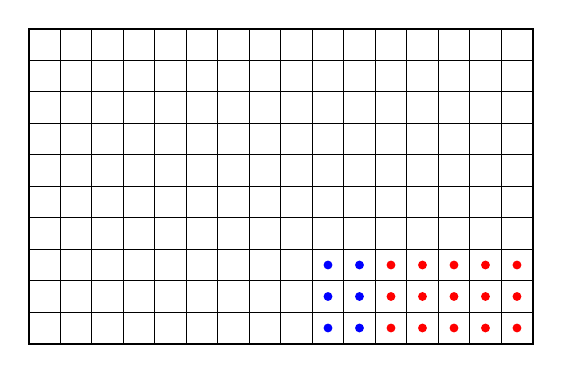
\begin{tikzpicture}[scale=0.4]
    % Grid
    \draw[step=1, thin, black] (0,0) grid (16,10);
    \draw[thick] (0,0) rectangle (16,10);
    % Red subregion
    \foreach \i in {11, 12, 13, 14, 15} {
        \foreach \j in {0, 1, 2} {
            \fill[red] (\i+0.5, \j+0.5) circle (4pt);
        }
    }
    
    % Blue subregion
    \foreach \i in {9, 10} {
        \foreach \j in {0, 1, 2} {
            \fill[blue] (\i+0.5, \j+0.5) circle (4pt);
        }
    }
\end{tikzpicture}
\begin{tikzpicture}[overlay, remember picture, scale=0.3]
  % Legend Box
  \begin{scope}[xshift=-20.8cm, yshift=16.8cm]
    \draw[thick] (-1,0.5) rectangle (6,-3);
   
    \fill[blue] (0,-0.5) circle (6pt); % Blue dot
    \node[align=left] at (3,-0.5) {Volume 1};
     
    \fill[red] (0,-2) circle (6pt);  % Red dot
    \node[align=left] at (3,-2) {Volume 2};
  \end{scope}
\end{tikzpicture}
\end{minipage}

\end{frame}

\begin{frame}\frametitle{\textit{meshdist}: \mirgecom{} Mesh Partitioning Utility}
  \begin{minipage}[t][.4\textheight][t]{\textwidth}
    %\begin{multicols}{2}
    \begin{itemize}
      \item $M$-decomp runs on $\text{NP} \le M$  (here $M=4$)
      \item Uses \textit{Metis} by default, 1dpart optional
      \item Mirrors built-in decomposition, \textbf{\textit{except}} writes:
        \begin{itemize}
        \item el-to-rank map: decomp.pkl     % $r_m[E_N]$   % (maps global element id $E_n$ to MPI rank $r_m$)
        \item el-to-partid map: mvdecomp.pkl (partid = (rank, vol)) % (maps global element id $E_N$ to PartID (rank, vol) pair
        \item $M$-partitioned mesh to pkl file per rank
        \end{itemize}
    \end{itemize}
  \end{minipage}
  \vspace{-20pt}
  \center{\texttt{python -m mpi4py meshdist.py -1 -n 4 -i box.msh -o box\_4p}}
  \begin{minipage}[b][.4\textheight][t]{\textwidth}
    \begin{tikzpicture}[overlay, remember picture, scale=0.3]
      \begin{scope}[yshift=-11cm, xshift=30pt]
        % Grid
        \draw[step=1, thin, black] (0,0) grid (16,10);
        \draw[thick] (0,0) rectangle (16,10);
    
        % Red subregion
        \foreach \i in {11, 12, 13, 14, 15} {
          \foreach \j in {0, 1, 2} {
            \fill[red] (\i+0.5, \j+0.5) circle (4pt);
          }
        }
    
        % Blue subregion
        \foreach \i in {9, 10} {
          \foreach \j in {0, 1, 2} {
            \fill[blue] (\i+0.5, \j+0.5) circle (4pt);
          }
        }
        \begin{scope}[xshift=30cm]
          % Partition 0
          \draw[step=1, thin, black] (0,0) grid (4,10);
          \draw[thick] (0,0) rectangle (4,10);
          \node[font=\bfseries, blue] at (2,9) {0};
    
          % Partition 1
          \begin{scope}[xshift=4.5cm]
            \draw[step=1, thin, black] (0,0) grid (4,10);
            \draw[thick] (0,0) rectangle (4,10);
            \node[font=\bfseries, blue] at (2,9) {1};
          \end{scope}
    
          % Partition 2 with blue and red subregions
          \begin{scope}[xshift=9cm]
            \draw[step=1, thin, black] (0,0) grid (4,10);
            \draw[thick] (0,0) rectangle (4,10);
            \foreach \j in {0, 1, 2} {
              \fill[blue] (1.5, \j+0.5) circle (4pt);
              \fill[blue] (2.5, \j+0.5) circle (4pt);
              \fill[red] (3.5, \j+0.5) circle (4pt);
            }
            \node[font=\bfseries, blue] at (2,9) {2};
          \end{scope}
    
          % Partition 3 with red subregion
          \begin{scope}[xshift=13.5cm]
            \draw[step=1, thin, black] (0,0) grid (4,10);
            \draw[thick] (0,0) rectangle (4,10);
            \foreach \j in {0, 1, 2} {
              \fill[red] (0.5, \j+0.5) circle (4pt);
              \fill[red] (1.5, \j+0.5) circle (4pt);
              \fill[red] (2.5, \j+0.5) circle (4pt);
              \fill[red] (3.5, \j+0.5) circle (4pt);
            }
            \node[font=\bfseries, blue] at (2,9) {3};
          \end{scope}
        \end{scope}
        % Coordinates for arrow
        \coordinate (leftGridCenter) at (8,5);
        \coordinate (rightGridCenter) at (38,5);
        
        % Arrow with text
        \draw[->, ultra thick] (leftGridCenter) -- node[midway, fill=white, text width=3cm, align=center] {\textit{meshdist}} (rightGridCenter);
      \end{scope}
    \end{tikzpicture}
  \end{minipage}
\end{frame}

\begin{frame}\frametitle{Run \mirgecom{} on $M$ MPI Ranks (Multivolume)}
   \begin{minipage}[t][.4\textheight][t]{\textwidth}
    %\begin{multicols}{2}
      \begin{itemize}
      \item Reads $M$-partitioned input mesh
      \item Initializes \textit{volume-specific} solution
      \item Each solution dump is 1 PKL file per MPI rank with:
        \begin{itemize}
        \item Volume-specific DOFArray sizes correspond to PartIDs
        \item Arbitrary data structures in I/O dictionary 
        \end{itemize}
      \end{itemize}
    %\end{multicols}
  \end{minipage}
  \vfill
  \center{\texttt{mpiexec -n 4 python -m mpi4py prediction.py -i run\_params.yaml --lazy}}
  \begin{minipage}[b][.4\textheight][t]{\textwidth}
    \begin{tikzpicture}[overlay, remember picture, scale=0.25]
      \begin{scope}[xshift=10pt]
      \node at (2cm, -14.5cm) (center) {};

      %\begin{scope}[shift={(center)}]  % yshift=-10cm]
      \begin{scope}[yshift=-12cm]
        % Partition 0
        \draw[step=1, thin, black] (0,0) grid (4,10);
        \draw[thick] (0,0) rectangle (4,10);
        \node[font=\bfseries, blue] at (2,9) {0};
        
        % Partition 1
        \begin{scope}[xshift=4.5cm]
          \draw[step=1, thin, black] (0,0) grid (4,10);
          \draw[thick] (0,0) rectangle (4,10);
          \node[font=\bfseries, blue] at (2,9) {1};
        \end{scope}
    
        % Partition 2 with blue and red subregions
        \begin{scope}[xshift=9cm]
          \draw[step=1, thin, black] (0,0) grid (4,10);
          \draw[thick] (0,0) rectangle (4,10);
          \foreach \j in {0, 1, 2} {
            \fill[blue] (1.5, \j+0.5) circle (4pt);
            \fill[blue] (2.5, \j+0.5) circle (4pt);
            \fill[red] (3.5, \j+0.5) circle (4pt);
          }
          \node[font=\bfseries, blue] at (2,9) {2};
        \end{scope}
    
        % Partition 3 with red subregion
        \begin{scope}[xshift=13.5cm]
          \draw[step=1, thin, black] (0,0) grid (4,10);
          \draw[thick] (0,0) rectangle (4,10);
          \foreach \j in {0, 1, 2} {
            \fill[red] (0.5, \j+0.5) circle (4pt);
            \fill[red] (1.5, \j+0.5) circle (4pt);
            \fill[red] (2.5, \j+0.5) circle (4pt);
            \fill[red] (3.5, \j+0.5) circle (4pt);
          }
          \node[font=\bfseries, blue] at (2,9) {3};
        \end{scope}
        \begin{scope}[xshift=40cm]
          % Partition (0,0)
          \draw[step=1, thin, black] (0,0) grid (4,10);
          \draw[thick] (0,0) rectangle (4,10);
          \node[font=\bfseries, blue] at (2,9) {(0,0)};

          % Partition (1,0)
          \begin{scope}[xshift=4.5cm]
            \draw[step=1, thin, black] (0,0) grid (4,10);
            \draw[thick] (0,0) rectangle (4,10);
            \node[font=\bfseries, blue] at (2,9) {(1,0)};
          \end{scope}

          % Partition (2,0) 
          \begin{scope}[xshift=9cm]
            \foreach \i in {0,1,2,3} {
              \foreach \j in {3,4,...,9} {
                \draw (\i,\j) rectangle (\i+1,\j+1);
              }
            }
            \draw (0,0) rectangle (1,3);
            \draw (0,0) rectangle (1,1);
            \draw (0,1) rectangle (1,2);
            \draw (0,2) rectangle (1,3);
            \draw[thick] (0,0) -- (1,0) -- (1,3) -- (4,3) -- (4,10) -- (0,10) -- cycle;
            \node[font=\bfseries, blue] at (2,9) {(2,0)};
          \end{scope}

          % Partition (2,1) with blue subregion
          \begin{scope}[xshift=13.5cm, yshift=6cm]
            \draw[step=1, thin, black] (0,0) grid (2,4);
            \draw[thick] (0,0) rectangle (2,4);
            \foreach \j in {0,1,2,3} {
              \fill[blue] (0.5, \j+0.5) circle (4pt);
              \fill[blue] (1.5, \j+0.5) circle (4pt);
            }
            \node[font=\bfseries, blue] at (1,3) {(2,1)};
          \end{scope}

          % Partition (2,2) with red subregion
          \begin{scope}[xshift=13.5cm, yshift=2cm]
            \draw[step=1, thin, black] (0,0) grid (1,3);
            \draw[thick] (0,0) rectangle (1,3);
            \foreach \j in {0,1,2} {
              \fill[red] (0.5, \j+0.5) circle (4pt);
            }
            \node[font=\bfseries, blue] at (0.5,2) {(2,2)};
          \end{scope}

          % Partition (3,0)
          \begin{scope}[xshift=16cm, yshift=3.5cm]
            \draw[step=1, thin, black] (0,0) grid (4,7);
            \draw[thick] (0,0) rectangle (4,7);
            \node[font=\bfseries, blue] at (2,6) {(3,0)};
          \end{scope}

          % Partition (3,2) with red subregion
          \begin{scope}[xshift=16cm, yshift=-0.5cm]
            \draw[step=1, thin, black] (0,0) grid (4,3);
            \draw[thick] (0,0) rectangle (4,3);
            \foreach \j in {0,1,2} {
              \fill[red] (0.5, \j+0.5) circle (4pt);
              \fill[red] (1.5, \j+0.5) circle (4pt);
              \fill[red] (2.5, \j+0.5) circle (4pt);
              \fill[red] (3.5, \j+0.5) circle (4pt);
            }
            \node[font=\bfseries, blue] at (2,2) {(3,2)};
          \end{scope}
        \end{scope}
        \begin{scope}[xshift=5cm]
          % Coordinates for arrow
          \coordinate (leftGridCenter) at (8,5);
          \coordinate (rightGridCenter) at (38,5);
        
          % Arrow with text
          \draw[->, ultra thick] (leftGridCenter) -- node[midway, fill=white, text width=3cm, align=center] {\textit{MIRGE-Com}} (rightGridCenter);
        \end{scope}
      \end{scope}
      \end{scope}
    \end{tikzpicture}
  \end{minipage}
\end{frame}

\begin{frame}\frametitle{\mirgecom{} I/O Datastructure}
  \begin{itemize}
  \item Arbitrary, user-defined I/O data from \mirgecom{}
  \item No reliable way to associate DOFArrays with PartIDs
  \item Really convenient; almost completely bonkers
  \end{itemize}
  \begin{tikzpicture}
    \begin{scope}[yshift=7pt, xshift=7pt]
      \node at (0,0) {\snippetboxbigtab{Figures/mtc/write_restart.py}{\href{https://github.com/illinois-ceesd/drivers_y3-prediction/blob/main/y3prediction/prediction.py}{prediction\_write\_restart}}};
    \end{scope}
\end{tikzpicture}
\end{frame}

\begin{frame}\frametitle{M-to-N Transfer with \textit{redist}}
  \begin{minipage}[t][.4\textheight][t]{\textwidth}
    \begin{multicols}{2}
      \begin{itemize}
      \item Input: $M$-data (\mirgecom{} restart pkl files), $M$-decomp, $N$-decomp
      \item Unbonks the restart data with kludges:
        \begin{itemize}
        \item Detect DOFArrays in restart data: Must find an $M$-partition with \textit{all} volumes
        \item Compares DOFArray sizes to $M$-part volume sizes for volume-to-DOFArray correspondence
        \end{itemize}
      \item Creates DOFArray index mapping: $M$-decomp-local $\rightarrow$ $N$-decomp-local
      \item Reads and copies necessary $M$-data pkl files to cover $N$-part elements
      \item Writes $N$-data (new \mirgecom{} restart pkl files)
      \item Runs on arbitrary resource, dividing work like \textit{meshdist} 
      \end{itemize}
    \end{multicols}
  \end{minipage}
  \vfill
  \center{\texttt{redist.py -m 4 -n 3 -i rst\_4p -s mesh\_4p -t mesh\_3p -o rst\_3p}}
  \begin{minipage}[b][.4\textheight][t]{\textwidth}
    \begin{tikzpicture}[overlay, remember picture, scale=0.25]
      \begin{scope}[yshift=10pt, xshift=20pt]
      \node at (2cm, -14.5cm) (center) {};

      %\begin{scope}[shift={(center)}]  % yshift=-10cm]
      \begin{scope}[yshift=-12cm]
        % Partition (0,0)
        \draw[step=1, thin, black] (0,0) grid (4,10);
        \draw[thick] (0,0) rectangle (4,10);
        \node[font=\bfseries, blue] at (2,9) {(0,0)};
        
        % Partition (1,0)
        \begin{scope}[xshift=4.5cm]
          \draw[step=1, thin, black] (0,0) grid (4,10);
          \draw[thick] (0,0) rectangle (4,10);
          \node[font=\bfseries, blue] at (2,9) {(1,0)};
        \end{scope}

        % Partition (2,0)
        \begin{scope}[xshift=9cm]
          \foreach \i in {0,1,2,3} {
            \foreach \j in {3,4,...,9} {
              \draw (\i,\j) rectangle (\i+1,\j+1);
            }
          }
          \draw (0,0) rectangle (1,3);
          \draw (0,0) rectangle (1,1);
          \draw (0,1) rectangle (1,2);
          \draw (0,2) rectangle (1,3);
          \draw[thick] (0,0) -- (1,0) -- (1,3) -- (4,3) -- (4,10) -- (0,10) -- cycle;
          \node[font=\bfseries, blue] at (2,9) {(2,0)};
        \end{scope}

        % Partition (2,1) with blue subregion
        \begin{scope}[xshift=13.5cm, yshift=6cm]
          \draw[step=1, thin, black] (0,0) grid (2,4);
          \draw[thick] (0,0) rectangle (2,4);
          \foreach \j in {0,1,2,3} {
            \fill[blue] (0.5, \j+0.5) circle (4pt);
            \fill[blue] (1.5, \j+0.5) circle (4pt);
          }
          \node[font=\bfseries, blue] at (1,3) {(2,1)};
        \end{scope}

        % Partition (2,2) with red subregion
        \begin{scope}[xshift=13.5cm, yshift=2cm]
          \draw[step=1, thin, black] (0,0) grid (1,3);
          \draw[thick] (0,0) rectangle (1,3);
          \foreach \j in {0,1,2} {
            \fill[red] (0.5, \j+0.5) circle (4pt);
          }
          \node[font=\bfseries, blue] at (0.5,2) {(2,2)};
        \end{scope}

        % Partition (3,0)
        \begin{scope}[xshift=16cm, yshift=3.5cm]
          \draw[step=1, thin, black] (0,0) grid (4,7);
          \draw[thick] (0,0) rectangle (4,7);
          \node[font=\bfseries, blue] at (2,6) {(3,0)};
        \end{scope}
        
        % Partition (3,2) with red subregion
        \begin{scope}[xshift=16cm, yshift=-0.5cm]
          \draw[step=1, thin, black] (0,0) grid (4,3);
          \draw[thick] (0,0) rectangle (4,3);
          \foreach \j in {0,1,2} {
            \fill[red] (0.5, \j+0.5) circle (4pt);
            \fill[red] (1.5, \j+0.5) circle (4pt);
            \fill[red] (2.5, \j+0.5) circle (4pt);
            \fill[red] (3.5, \j+0.5) circle (4pt);
          }
          \node[font=\bfseries, blue] at (2,2) {(3,2)};
        \end{scope}
        \begin{scope}[xshift=40cm]
          % Partition (0,0)
          \draw[step=1, thin, black] (0,0) grid (5,10);
          \draw[thick] (0,0) rectangle (5,10);
          \node[font=\bfseries, orange] at (2.5,9) {(0,0)};

          % Partition (1,0) (panhandle grid)
          \begin{scope}[xshift=5.5cm]
            \foreach \i in {0,1,2,3,4} {
              \foreach \j in {3,4,...,9} {
                \draw (\i,\j) rectangle (\i+1,\j+1);
              }
            }
            \foreach \i in {0,1,2} {
              \foreach \j in {0,1,2} {
                \draw (\i,\j) rectangle (\i+1,\j+1);
              }
            }
            \draw[thick] (0,0) -- (3,0) -- (3,3) -- (5,3) -- (5,10) -- (0,10) -- cycle;
            \node[font=\bfseries, orange] at (2.5,9) {(1,0)};
          \end{scope}

          % Partition (1,1) with blue subregion
          \begin{scope}[xshift=9cm, yshift=-0.5cm]
            \draw[step=1, thin, black] (0,0) grid (2,3);
            \draw[thick] (0,0) rectangle (2,3);
            \foreach \j in {0,1,2} {
              \fill[blue] (0.5, \j+0.5) circle (4pt);
              \fill[blue] (1.5, \j+0.5) circle (4pt);
            }
            \node[font=\bfseries, orange] at (1,2) {(1,1)};
          \end{scope}

          % Partition (2,0)
          \begin{scope}[xshift=12cm, yshift=3cm]
            \draw[step=1, thin, black] (0,0) grid (6,7);
            \draw[thick] (0,0) rectangle (6,7);
            \node[font=\bfseries, orange] at (3,6) {(2,0)};
          \end{scope}

          % Partition (2,2) with red subregion
          \begin{scope}[xshift=12cm, yshift=-0.5cm]
            \draw[step=1, thin, black] (0,0) grid (6,3);
            \draw[thick] (0,0) rectangle (6,3);
            \foreach \j in {0,1,2} {
              \fill[red] (0.5, \j+0.5) circle (4pt);
              \fill[red] (1.5, \j+0.5) circle (4pt);
              \fill[red] (2.5, \j+0.5) circle (4pt);
              \fill[red] (3.5, \j+0.5) circle (4pt);
              \fill[red] (4.5, \j+0.5) circle (4pt);
              \fill[red] (5.5, \j+0.5) circle (4pt);
            }
            \node[font=\bfseries, orange] at (3,2) {(2,2)};
          \end{scope}
        \end{scope}
        \begin{scope}[xshift=8cm]
          % Coordinates for arrow
          \coordinate (leftGridCenter) at (8,5);
          \coordinate (rightGridCenter) at (38,5);
        
          % Arrow with text
          \draw[->, ultra thick] (leftGridCenter) -- node[midway, fill=white, text width=3cm, align=center] {\textit{redist}} (rightGridCenter);
        \end{scope}
      \end{scope}
      \end{scope}
    \end{tikzpicture}
  \end{minipage}
\end{frame}

\begin{frame}\frametitle{TODOs For M-to-N}
  \begin{itemize}
  \item Everything is in \mirgecom{} PR 973 (WIP)
  \item Some things are prediction-specific (gmsh mesh source)
  \item Unkludge the restart debonk (some sort of standardization):
    \begin{itemize}
    \item Auto-detection of DOFArrays in restart data is OK - could be better
    \item Finding partition with all volumes, ugh
    \item Need some way to associate DOFArrays $\rightarrow$ Volume/dd
    \end{itemize}
  \item \textit{Meshmode} support for m-to-n mappings would be nice 
  \end{itemize}
\end{frame}

\input{../ceesd-acknowledgement.tex}

\end{document}
